\chapter{Конструкторская часть}
В данной части будут реализованы блок-схемы алгоритмов поиска максимального числа в последовательности, произведена оценка их трудоёмкости и затрачиваемая памяти.

\section{Описание алгоритмов}
Оба алгоритма предназначены для нахождения максимального элемента последовательности. Входными данными служит массив целых чисел и его размер, содержащий минимум 1 элемент. Выходные данные: максимальный элемент массива.

На рисунке \ref{fig:risunok_1} изображена схема итеративного алгоритма. На рисунке \ref{fig:risunok_2}  изображена схема рекурсивного алгоритма.


\begin{figure}[H]
	\centering
	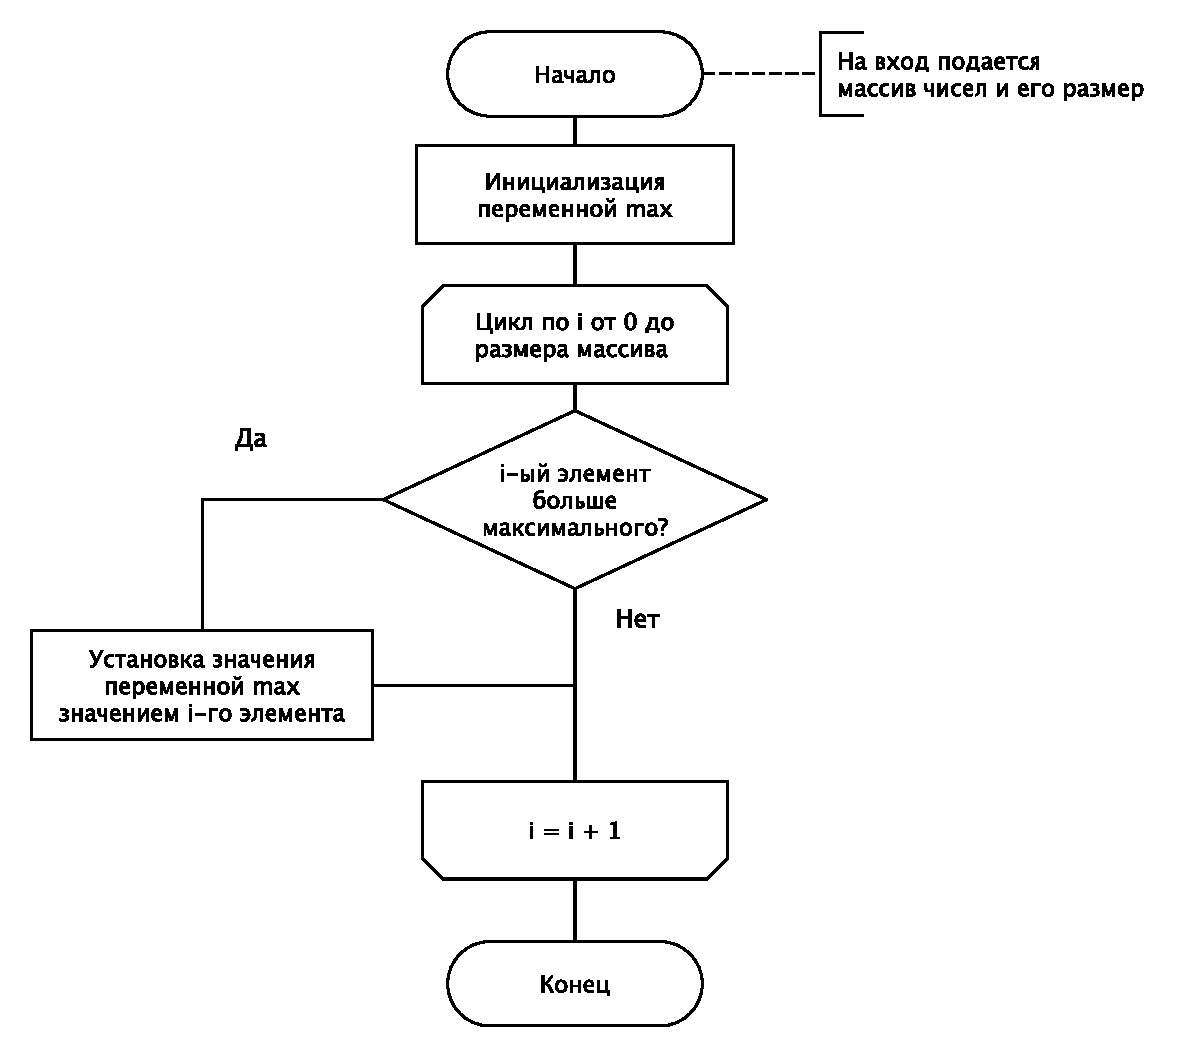
\includegraphics[width=1\textwidth]{images/AA2_1.pdf}
	\caption{Схема итерационного алгоритма нахождения максимального элемента массива}
	\label{fig:risunok_1}
\end{figure}

\begin{figure}[H]
	\centering
	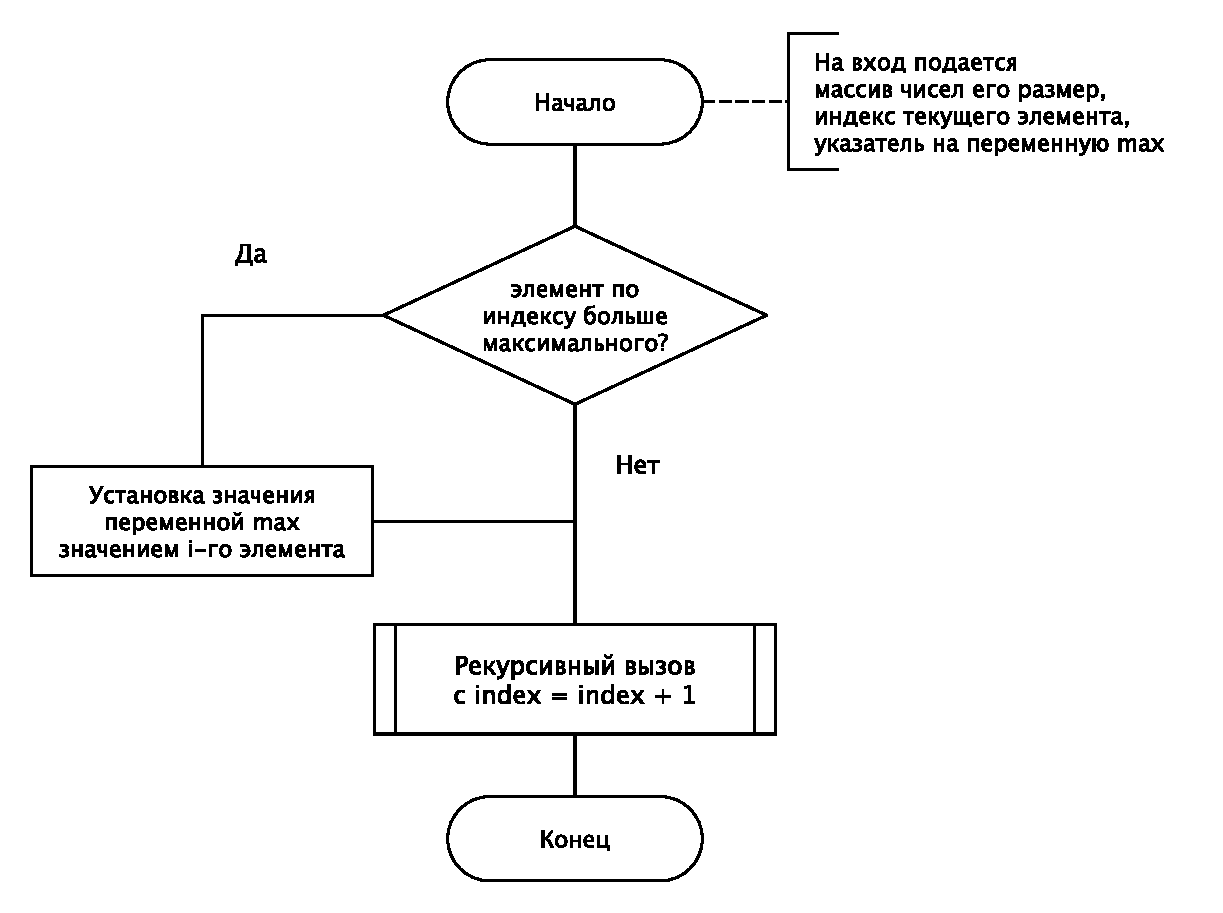
\includegraphics[width=1\textwidth]{images/AA2_2.pdf}
	\caption{Схема рекурсивного алгоритма нахождения максимального элемента массива}
	\label{fig:risunok_2}
\end{figure}


\section{Оценка трудоёмкости алгоритмов}
\subsection{Модель вычислений}
Была введена следующая модель вычислений:
    \begin{itemize}
	\itemтрудоёмкость следующих операций равной 1:\\
	\( + \), \( - \), \( ! \), \( != \), \( == \), \( \neq \), \( \leq \), \( \geq \), \( > \), \( < \), \( += \), \( -= \), \( []\), \( || \), \( \&\& \), \( << \)
	\itemтрудоёмкость следующих операция равной 2:\\
	\( * \), \( / \), \( *= \), \( /= \), \( \% \)
\end{itemize}

Трудоёмкость условного оператора определим:
\begin{equation}
	f_{\text{if}} = f_{\text{условия}} +
	\begin{cases}
		\min(f_{\text{true}}, f_{\text{false}}), & \text{в лучшем случае} \\
		\max(f_{\text{true}}, f_{\text{false}}), & \text{в худшем случае}
	\end{cases}
\end{equation}

Трудоёмкость цикла определяется как:
\begin{equation}
	f_{\text{цикл}} = f_{\text{иниц.}} + f_{\text{усл.}} + n \cdot (f_{\text{тела}} + f_{\text{инк.}} + f_{\text{усл.}})
\end{equation}

Для анализа трудоёмкости применяется метод, основанный на исследовании дерева вызовов рекурсии[4]. Согласно подходу, общая трудоёмкость рекурсивного алгоритма A на входных данных D складывается из компонент:
\begin{equation}
	f = f_{R(D)} + f_{C(D)}
		\label{eq:2.3}
\end{equation}
где:
\begin{itemize}\item $f$ — суммарная трудоёмкость алгоритма;
	\item $f_{R(D)}$ — затраты на организацию и обслуживание рекурсивных вызовов;
	\item $f_{C(D)}$ — трудоёмкость продуктивных вычислений.
 \end{itemize}

Накладные расходы определяются количеством узлов в дереве рекурсии и стоимостью одного вызова:
\begin{equation}
	f_{R(D)} = R(D) \cdot f_{R(1)}
	\label{eq:2.4}
\end{equation}
где:
\begin{itemize}
	\item $R(D)$ — число вершин дерева рекурсии;
	\item $f_{R(1)}$ — трудоёмкость входа в функцию и возврата.
\end{itemize}

Стоимость рекурсивного вызова и возврата оценивается по формуле:
\begin{equation}
	f_{R(1)} = 2 \cdot (p + k + r + f + l + 1)
	\label{eq:2.5}
\end{equation}
где:
\begin{itemize}
	\item $p$ — число передаваемых параметров;
	\item $k$ — количество значение, возвращаемых по ссылке;
	\item $r$ — число регистров процессора, сохраняемых в стеке;
	\item $f$ — 1, если есть возврат, 0 если нету;
	\item $i$ — количество локальных переменных.
\end{itemize}


Продуктивные вычисления делятся на действия, выполняемые во внутренних узлах дерева и действиях в листьях:
\begin{equation}
	f_{C(D)} = f_{CV(D)} + f_{CL(D)}
\end{equation}
где:
\begin{itemize}
	\item $f_{CV(D)}$ — трудоёмкость во внутренних вершинах;
	\item $f_{CL(D)}$ — трудоёмкость в листьях.
\end{itemize}

Трудоёмкость в листьях расчитывается следующим способом:
\begin{equation}
	f_{CL(D)} = R_{L(D)} + f{CL(1)}
	\label{eq:2.7}
\end{equation}
где:
\begin{itemize}
	\item $R_{L(D)} $ — число листьев дерева рекурсии;
	\item $f{CL(1)}$ — вычислительная сложность при завершении рекурсии (обработка базового случая).
\end{itemize}

В общем случае трудоёмкость во внутренних вершинах определяется суммированием по всему дереву:
\begin{equation}
	f_{CV}(D) = \sum_{m=1}^{H_R(D)-1} \sum_{k=1}^{K(m)} f_{CV}(v_{mk})
		\label{eq:2.8}
\end{equation}
где:
\begin{itemize}
	\item $H_R(D) $ — максимальная глубина рекурсии;
	\item $K(m)$ — количество внутренних вершин на уровне $m$;
	\item $v_{mk}$ — $k$-я вершина на этом уровне.
\end{itemize}

Подставив формулу \ref{eq:2.4}, \ref{eq:2.7}, \ref{eq:2.8} в выражение \ref{eq:2.3}, получится общая формула трудоёмкости рекурсивного алгоритма:
\begin{equation}
f_A(D) = R(D) \cdot f_{R(1)} + R_L(D) \cdot f_{CL}(1) + \sum_{m=1}^{H_R(D)-1} \sum_{k=1}^{K(m)} f_{CV}(v_{mk}).
\label{eq:2.9}
\end{equation}


В частном случае, когда продуктивные вычисления одинаковы во всех узлах, формула упрощается. Пусть $R_V(D)$ — число внутренних вершин, а $f_{CV}(v)$ — постоянная трудоёмкость одного внутреннего узла. Тогда:
\begin{equation}
	f_{CV(D)} = R_{V(D)} \cdot f_{CV(v)}
\end{equation}
и в итоге, оценка трудоёмкости принимает вид:
\begin{equation}
	f_A(D) = R(D) \cdot f_{R(1)} + R_L(D) \cdot f_{CL}(1) + R_V(D) \cdot f_{CV}(v).
\end{equation}



\subsection{Трудоёмкость итеративного алгоритма}
Выделяются два случая: в лучшем случае, обменов происходить не будет, и таким образом, трудоёмкость можно получить следующим способом:
\begin{equation}
	f = f_{\text{инициализации}} + f_{\text{условия}} + n \cdot (f_{\text{тела}} + f_{\text{инкремента}} + f_{\text{условия}})
\end{equation}
\begin{equation}
	f = 1 + 1 + n \cdot (2 + 1 + 1)
\end{equation}
\begin{equation}
	f = 2 + 4n
\end{equation}

А в худшем случае:
\begin{equation}
	f = f_{\text{инициализации}} + f_{\text{условия}} + n \cdot (f_{\text{тела}} + f_{\text{инкремента}} + f_{\text{условия}})
\end{equation}
\begin{equation}
	f_{\text{тела}} = 	f_{\text{условия}} + f_{\text{тела\_цикла}} = 4
 \end{equation}
\begin{equation}
	f = 1 + 1 + n \cdot (4 + 1 + 1)
\end{equation}
\begin{equation}
	f = 2 + 6n
\end{equation}

\subsection{Трудоёмкость рекурсивного алгоритма}
Для рекурсивного алгоритма трудоёмкость обслуживание одного вызова определяется по формуле \ref{eq:2.5}
\begin{equation}
	f_{R(1)} = 2 \cdot (1 + 1 + 0 + 0 + 0 + 1) = 6
\end{equation}

Трудоёмкость в листе дерева считается по формуле \ref{eq:2.20}
\begin{equation}
f_{CL} = 1
\label{eq:2.20}
\end{equation}

Трудоёмкость во внутреннем узле дерева считается по формуле \ref{eq:2.21}
\begin{equation}
	f_{CV} = 5
	\label{eq:2.21}
\end{equation}

Общая трудоёмкость рекурсивного алгоритма находится по формуле \ref{eq:2.22}
\begin{equation}
	f_{\text{рекурсии}} = 6 * N + 1 * 4 + (N - 1) * 5 = 11N - 1
	\label{eq:2.22}
\end{equation}


\section{Оценка затрачиваемой памяти}
\subsection{Итеративный алгоритм}
Итеративная реализация алгоритма не требует выделения дополнительной памяти, таким образом. Определим что, $V$ это мера затрачиваемой памяти, тогда:
\begin{equation}
	V_\text{{итерационного}} = 1
\end{equation}

\subsection{Рекурсивный алгоритм}
Рекурсивная реализация алгоритма хранит состояние каждого вызова в аппаратном стеке. Объем используемой памяти прямо-пропорционален глубине рекурсии. Размер одного кадра стека определяется количеством данных, сохраняемым при каждом вызове. Согласно методике[4], объем кадра вычисляется по формуле \ref{eq:Vkadr}: 
 \begin{equation}
 	V_{\text{кадра}} = p + k + r + f + l + 1,
	\label{eq:Vkadr}
 \end{equation}
 где:

\begin{itemize}
\item $p$ — число передаваемых параметров;
\item $k$ — количество значений, возвращаемых по ссылке;
\item $r$ — число сохраняемых регистров процессора;
\item $f = 1$, если функция, и $f = 0$ если процедура);
\item $l$ — количество локальных переменных;
\item $1$ — ячейка для хранения адреса возврата.
\end{itemize}
 
 Подставляя значения в формулу \eqref{eq:Vkadr}, получим:
 \begin{equation}
 	V_{\text{кадра}} = 1 + 1 + 1 + 0 + 0 + 1 = 4
 \end{equation}
 
Во всех случаях рекурсия достигнет своей максимальной глубины, равной длине массива. Тогда объем дополнительной памяти будет равен произведению размера кадра на глубину рекурсии.
 \begin{equation}
 	V_{\text{рекурсии}} = 4 * N
 \end{equation}
 


\section{Используемые типы данных}
При реализации алгоритмов использовались следующие типы данных:
\begin{itemize}
	\itemразмер массива: \text{size\_t};
	\itemтип данных массива: int;
\end{itemize}


\section{Структура программы}
Программное обеспечение будет состоять из нескольких частей:
\begin{itemize}
	\itemглавный модуль — предоставляет возможность выбора режима работы программы, а также обеспечивает запуск программы;
	\itemинтерфейс — модуль для взаимодействия пользователя с программой. Пользователь может выбрать режим работы, а также ввести входные данные для поиска максимального элемента массива или тестовых замеров;
	\itemмодуль, содержащий функции для работы с массивами — предоставляет возможность объявить, проинициализировать, прочитать с терминала, и заполнить случайными числам;
	\itemмодуль для совершения замеров процессорного времени выполнения поиска максимального числа;
\end{itemize}

\section*{Вывод}
На основе аналитической части были реализованы блок-схемы алгоритмов поиска максимального числа массива, произведена оценка их трудоёмкости и затрачиваемой памяти, а также продуманы модули программы.
\clearpage
